\documentclass[prb,superscriptaddress,showpacs,twocolumn,letterpaper]{revtex4}
\usepackage{amsmath}
\usepackage{graphicx}
\usepackage[backref,colorlinks,linkcolor=blue,citecolor=blue]{hyperref}


\pacs{78.68.+m, 42.65.An, 71.15.Mb, 42.65.Ky, 78.66.-w}


\begin{document}

\title{Improved \emph{ab initio} calculation of surface second-harmonic
generation from Si(111)(1$\times$1):H}

\author{Sean M. Anderson}
    \affiliation{Centro de Investigaciones en \'Optica, 
                Le\'on, Guanajuato, M\'exico}
\author{Nicolas Tancogne-Dejean}
    \affiliation{Laboratoire des Solides Irradi\'es, \'Ecole Polytechnique, 
                CNRS, CEA/DSM, 91128 Palaiseau, France}
    \affiliation{Max Planck Institute for the Structure and Dynamics of Matter, 
                 Luruper Chaussee 149, D-22761 Hamburg, Germany}
    \affiliation{European Theoretical Spectroscopy Facility (ETSF), 
                Palaiseau, France}
\author{Bernardo S. Mendoza}\email{bms@cio.mx}
    \affiliation{Centro de Investigaciones en \'Optica, 
                Le\'on, Guanajuato, M\'exico}
\author{Val\'erie V\'eniard}
    \affiliation{Laboratoire des Solides Irradi\'es, \'Ecole Polytechnique, 
                CNRS, CEA/DSM, 91128 Palaiseau, France}
    \affiliation{European Theoretical Spectroscopy Facility (ETSF), 
                Palaiseau, France}

\begin{abstract}
We carry out an improved \emph{ab initio} calculation of surface second-harmonic
generation from the Si(111)(1$\times$1):H surface. This calculation includes
three new features in one unique formulation: (i) the scissors correction, (ii)
the contribution of the nonlocal part of the pseudopotentials, and (iii) the
inclusion of a cut function to extract the surface response, all within the
independent particle approximation. We apply these improvements on the
Si(111)(1$\times$1):H surface and compare with various experimental spectra from
several different sources. We also revisit the three layer model for the SSHG
yield and demonstrate that it provides more accurate results over several, more
common, two layer models. We demonstrate the importance of using properly
relaxed coordinates for the theoretical calculations. We conclude that this new
approach to the calculation of the second-harmonic spectra is versatile and
accurate within this level of approximation. This well-characterized surface
offers an excellent platform for comparison with theory, and allows us to offer
this study as an efficient benchmark for this type of calculation.
\end{abstract}


\maketitle


\section{Introduction}\label{sec:intro}

Surface second-harmonic generation (SSHG) has been shown to be an effective,
nondestructive and noninvasive probe to study surface and interface
properties.\cite{bloembergenAPB99, chenPRL81, daumPRL93, downerPSSA01,
downerSIA01, hughesPRB96, mcgilpOE94, mcgilpSRL99, mendozaPRL98, shenNAT89} SSHG
experiments are now very cost-effective and popular because they provide easy
access to buried interfaces and nanostructures, and interest in these techniques
continues to increase with the advent of ultrathin and bidimensional
materials.\cite{deanPRB14, malardPRB13} The high surface sensitivity of SSHG
spectroscopy is due to the fact that within the dipole approximation, the bulk
second-harmonic generation (SHG) in centrosymmetric materials is identically
zero. The SHG process can occur only at the surface where the inversion symmetry
is broken.

There are several theoretical formalisms that describe the SHG process for
surfaces with different approximations and varying levels of
difficulty.\cite{levinePRB94,mendozaPRL98, arzatePRB01, mendozaPRB01,
mejiaPRB02, sanoPRB02, mejiaRMF04, trollePRB14} In this paper, we focus on a
recent approach developed by us in Ref. \onlinecite{andersonPRB15}. It includes
three features not previously found in a single formulation: (i) the scissors
correction, (ii) the contribution of the nonlocal part of the pseudopotentials,
and (iii) the cut function used to extract the surface response, all within the
independent particle approximation. The inclusion of these three contributions
opens the possibility to study SSHG with more versatility and accuracy than was
previously available at this level of approximation. We also use the three layer
(3-layer) model for the SSHG yield, which considers that the SH conversion takes
place in a thin layer just below the surface that lies under the vacuum region
and above the bulk of the material. Validating these improvements is difficult,
however, without experimental data for comparison.

SSHG experiments focusing on semiconductor surfaces are available, but they are
often reported over very limited energy ranges and lacking units and scale for
the intensity. This lack of comprehensive experimental data has made comparison
between theory and experiment difficult. However, the Si(111)(1$\times$1):H
surface offers some respite in this area. This surface can be prepared to a high
degree of structural quality and has been experimentally characterized with SHG
to a great degree of accuracy.\cite{mitchellSS01, mejiaPRB02} The added H
saturates the surface Si dangling bonds and eliminates any surface-related
electronic states in the band gap. We consider that this surface represents an
ideal benchmark for \emph{ab initio} SSHG studies. More specifically, SSHG from
the Si(111)(1$\times$1):H surface was treated in detail in Ref.
\onlinecite{mejiaPRB02}, and their approach yielded good qualitative results.
However, the expressions presented for the nonlinear susceptibility tensor,
$\boldsymbol{\chi}(-2\omega;\omega,\omega)$, which is required for the SSHG
yield, are derived in the velocity gauge. This method incorrectly implements the
scissors quasiparticle correction and diverges for low
energies.\cite{cabellosPRB09} They also propose a two layer (2-layer) model for
SSHG which does not accurately represent the real physical process for surfaces.
We consider that the theoretical and computational aspects of this subject have
evolved considerably since then, making this topic ripe for revision.

In this paper, we present a comparison between theory and experiment by
presenting the improved theoretical calculations against experimental SSHG
spectra from several sources, namely Refs. \onlinecite{hoferAPA96,
bergfeldPRL04, mejiaPRB02, mitchellSS01}, with two-photon energies ranging from
2.5\,eV to 5\,eV covering both the E$_{1}$ and E$_{2}$ critical point
transitions for bulk Si. These SHG experiments were carried out with different
polarizations of incoming and outgoing beams which are taken into account in the
theoretical analysis. We find that the new formalism compares favorably with
experiment and permits insight into the physics behind SSHG. In spite of the
advances mentioned, our treatment neglects local field and excitonic effects
that are challenging from both a theoretical and a computational standpoint.
This topic merits further review and may prove to be crucial for more accurate
SSHG theory.

This paper is organized as follows. In Sec. \ref{sec:yield}, we present the
relevant equations and theory that describe the SSHG yield. In Sec.
\ref{sec:tensor}, we present the components of the nonlinear second-order
susceptibility tensor, $\boldsymbol{\chi}(-2\omega;\omega,\omega)$ which are
needed to calculate the SSHG yield. We describe our methodology and final
parameters for these calculations in Sec. \ref{sec:method}. In Sec.
\ref{sec:results}, we show the results of the comparison between our improved
formalism with the experimental spectra for the Si(111)(1$\times$1):H surface.
Finally, in Sec. \ref{sec:conclusions}, we present our conclusions and final
remarks.


\section{SSHG yield}\label{sec:yield}

We will briefly describe the 3-layer model for the SSHG yield in
this section. We mention that the formulas presented in Ref.
\onlinecite{mejiaPRB02}, where the 3-layer model was introduced for
the first time, have some minor mistakes that have been corrected in Ref.
\onlinecite{andersonARXIV16}. These revised formulas are what we use in this
article and are presented below. We assume that the fundamental electric field
at $1\omega$ induces the second-harmonic conversion in a thin layer just below
the surface described by a surface dielectric function,
$\boldsymbol{\epsilon}_{\ell}(\omega)$. This layer is below the vacuum region
and above the material bulk that is described by the bulk dielectric function,
$\boldsymbol{\epsilon}_b(\omega)$, as depicted in Fig.
\ref{fig:3layer}. In this surface layer, the nonlinear polarization
\begin{equation}\label{eq:polar}
\mathcal{P}^{\mathrm{a}}(2\omega) = 
\chi^{\mathrm{abc}}(-2\omega;\omega,\omega)
E^{\mathrm{b}}(\omega)E^{\mathrm{c}}(\omega)
\end{equation}
produces the SSHG that radiates into the vacuum where the measurements take
place. In Eq. \eqref{eq:polar}, $\mathbf{E}(\omega)$ is the fundamental electric
field, and there is a sum over the repeated Cartesian indices. In this model,
the SSHG yield is given by\cite{andersonARXIV16}
\begin{equation}\label{eq:r19}
\mathcal{R}_{iF}=
\frac{\omega^{2}}{2\epsilon_{0}c^{3}\cos^{2}\theta}
\left|\Gamma^{\ell}_{iF}\,r^{\ell}_{iF}\right|^2,
\end{equation}
where $\theta$ is the angle of incidence, $c$ the speed of light, and
$\epsilon_{0}$ the vacuum permittivity. The $i$ subscript denotes the incoming
$1\omega$ photon polarization and can be either $p$ or $s$. Analogously, the $F$
subscript is the polarization of the outgoing $2\omega$ photon, which we
represent with capital letters as either $P$ or $S$. Eq. \eqref{eq:r19} is
written in the MKS system of units, although the calculated SSHG yield is
reported in $\text{cm}^{2}/\text{W}$.

The $\Gamma^{\ell}_{iF}$ term contains the Fresnel factors for each polarization
case, and they are given by
\begin{align*}
\Gamma^{\ell}_{pP} &=
\frac{T^{v\ell}_{p}(\omega)T^{\ell b}_{p}(\omega)}
     {\sqrt{\varepsilon_{\ell}(\omega)}\varepsilon_{\ell}({2\omega})
     \sqrt{\varepsilon_{b}(2\omega)}}
\left[\frac{t^{v\ell}_{p}(\omega)t^{\ell b}_{p}(\omega)}
{\varepsilon_{\ell}(\omega)\sqrt{\varepsilon_{b}(\omega)}}\right]^{2},\\
\Gamma^{\ell}_{pS} &=
\frac{T^{v\ell}_{s}(\omega)T^{\ell b}_{s}(\omega)}
     {\sqrt{\varepsilon_{\ell}(\omega)}}
\left[\frac{t^{v\ell}_{p}(\omega)t^{\ell b}_{p}(\omega)}
      {\varepsilon_{\ell}(\omega)\sqrt{\varepsilon_{b}(\omega)}}\right]^{2},\\
\Gamma^{\ell}_{sP} &=
\frac{T_{p}^{v\ell}(\omega)T^{\ell b}_{p}(\omega)}
    {\sqrt{\varepsilon_{\ell}(\omega)}\varepsilon_{\ell}(2\omega)
    \sqrt{\varepsilon_{b}(2\omega)}}
\left[t_s^{v\ell}(\omega)t^{\ell b}_s(\omega)\right]^2,
\end{align*}
where $\varepsilon_{\ell}(\omega)$ is the average value of the layer dielectric
function, and the $v\ell$ and $\ell b$ superscripts denote either the
vacuum-layer or layer-bulk interfaces. The required Fresnel factors
are\cite{mizrahiJOSA88}
\begin{align*}
t_{p}^{\alpha\beta}(\omega) &=
\frac{2k_{\alpha}(\omega)
\sqrt{\varepsilon_{\alpha}(\omega)\varepsilon_{\beta}(\omega)}}
{k_{\alpha}(\omega)\varepsilon_{\beta}(\omega)+
k_{\beta}(\omega)\varepsilon_{\alpha}(\omega)},\\
t_s^{\alpha\beta}(\omega) &=
\frac{2k_{\alpha}(\omega)}{k_{\alpha}(\omega)+k_{\beta}(\omega)},\\
\end{align*}
where $k_{\alpha}(\omega) = [\varepsilon_{\alpha}(\omega)-\sin^2\theta]^{1/2}$
is the magnitude of the wavevector perpendicular to the surface divided by
$\omega/c$, and $\varepsilon_{v}(\omega) = 1$. The Fresnel factors denoted with
capital $T$ can be expressed as $T^{\alpha\beta}_{i}(\omega) =
t^{\alpha\beta}_{i}(2\omega)$, where $i$ can be either $s$ or $p$ polarization,
and $\alpha\beta$ can be either the vacuum-layer $(v\ell)$ or layer-bulk $(\ell
b)$ interface. For the remainder of this section, terms represented with capital
letters will be evaluated at $2\omega$. We shall also omit the ($\omega$) and
($2\omega$) dependence on some terms for ease of notation.

\begin{figure}[t]
\centering 
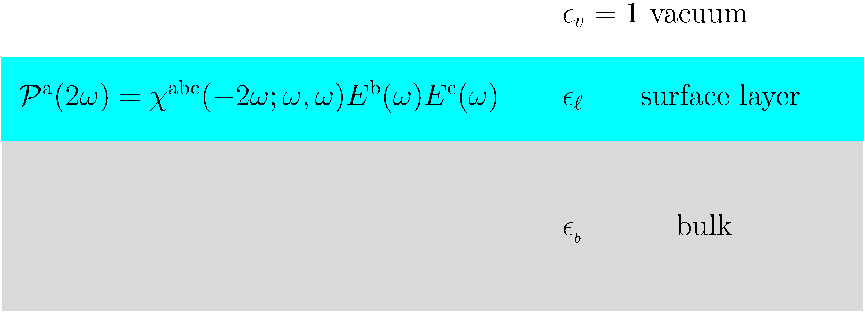
\includegraphics[width=0.48\textwidth]{plots/fig1}
\caption{(Color online) Representation of the 3-layer model for SSHG. Vacuum is
on top with $\varepsilon_{v}=1$; the layer with nonlinear polarization
$\mathcal{P}^{\mathrm{a}}(2\omega) =
\chi^{\mathrm{abc}}(-2\omega;\omega,\omega)
E^{\mathrm{b}}(\omega)E^{\mathrm{c}}(\omega)$ is characterized with
$\varepsilon_{\ell}(\omega)$ and the bulk with $\varepsilon_{b}(\omega)$. In the
dipole approximation, the bulk does not radiate
second-harmonic.\label{fig:3layer}}
\end{figure}

The 3-layer model described here can be reduced to the
2-layer,\cite{mizrahiJOSA88, sipePRB87,bloembergenPR62} that had been
traditionally used to study the SSHG yield. For this reduction, we consider that
$\boldsymbol{\mathcal{P}}(2\omega)$ is evaluated in the vacuum region, while the
fundamental fields are evaluated in the bulk region. To do this, we take the
$2\omega$ radiations factors for vacuum by taking $\ell=v$ (thus
$\varepsilon_{\ell}(2\omega)=1$, $T^{\ell v}_{i}=1$, $T^{\ell
b}_{i}=T^{vb}_{i}$) and the fundamental field inside medium $b$ by taking
$\ell=b$ (thus $\varepsilon_{\ell}(\omega)=\varepsilon_{b}(\omega)$,
$t^{v\ell}_{i}=t^{vb}_{i}$, and $t^{\ell b}_{i}=1$). This reduces Eq.
\eqref{eq:r19} to the equivalent expression in Refs. \onlinecite{mizrahiJOSA88}
and \onlinecite{sipePRB87}. Since $\boldsymbol{\mathcal{P}}(2\omega)$ is
evaluated in the vacuum we label this model as the 2-layer-vacuum model.


A third possibility that we consider is to take both
$\boldsymbol{\mathcal{P}}(2\omega)$ and the fundamental fields inside the bulk
of the material. The 3-layer model can be reduced by taking $\ell=b$, thus
$\varepsilon_{\ell}(2\omega)=\varepsilon_{b}(2\omega)$,
$T^{v\ell}_{i}=T^{b\ell}_{i}$, $T^{\ell b}_{i}=1$, and,
$\varepsilon_{\ell}(\omega)=\varepsilon_{b}(\omega)$,
$t^{v\ell}_{i}=t^{vb}_{i}$, and $t^{\ell b}_{i}=1$. In this case,
$\boldsymbol{\mathcal{P}}(2\omega)$ is evaluated in the bulk, thus we label this
model as the 2-layer-bulk model. We will compare all three of these models in
subsequent sections to determine which one more accurately describes the SSHG
yield. We summarize these models in Table
\ref{tab:models}.

\begin{table}[b]
\begin{ruledtabular}
\begin{tabular}{ l c c }
Label         &  $\boldsymbol{\mathcal{P}}(2\omega)$  &  $\mathbf{E}(\omega)$ \\
\hline
3-layer         &           $\ell$          &      $\ell$   \\
2-layer-vacuum  &            $v$            &        $b$    \\
2-layer-bulk    &            $b$            &        $b$    
\end{tabular}
\end{ruledtabular}
\caption{Summary of SSHG yield models. ``Label'' is the name used in subsequent
figures, while the remaining columns show in which medium we will consider the
specified quantity. $\ell$ is the thin layer below the surface of the material,
$v$ is the vacuum region, and $b$ is the bulk region of the material. Note that
the ``vacuum'' or ``bulk'' tag in the label refers to the layer in which
$\boldsymbol{\mathcal{P}}(2\omega)$  is evaluated.
\label{tab:models}}
\end{table}


The Si(111)(1$\times$1):H surface is in symmetry group $C_{3v}$ and has the
following nonzero components\cite{sipePRB87} of the nonlinear susceptibility
tensor, $\boldsymbol{\chi}(-2\omega;\omega,\omega)$:
\begin{align*}
\chi^{zzz}&\equiv\chi_{\perp\perp\perp},\nonumber\\
\chi^{zxx}&=\chi^{zyy}\equiv\chi_{\perp\parallel\parallel},\nonumber\\
\chi^{xxz}&=\chi^{yyz}\equiv\chi_{\parallel\parallel\perp},\nonumber\\
\chi^{xxx}&=-\chi^{xyy}=-\chi^{yyx}\equiv\chi_{\parallel\parallel\parallel}.
\end{align*}
We have chosen the $x$ and $y$ axes along the $[11\overline{2}]$ and
$[1\overline{1}0]$ directions. The $(-2\omega;\omega,\omega)$ term has been
omitted for ease of notation. These tensor components will be given in Sec.
\ref{sec:tensor}. We are interested in $\mathcal{R}_{pP}$, $\mathcal{R}_{pS}$,
and $\mathcal{R}_{sP}$ for our comparison with experiment, so we write the
remaining terms of Eq. \eqref{eq:r19} as
\begin{align}
r^{\ell}_{pP} &= \varepsilon_{b}(2\omega)\sin\theta
\bigl[\varepsilon^{2}_{b}(\omega)\sin^{2}\theta\,\chi_{\perp\perp\perp} 
+ \varepsilon^{2}_{\ell}(\omega)k^{2}_{b}\,\chi_{\perp\parallel\parallel}\bigr]
\nonumber\\
&- \varepsilon_{\ell}(\omega)\varepsilon_{\ell}(2\omega)
k_{b}K_{b}\bigl[2\sin\theta\varepsilon_{b}(\omega)
\,\chi_{\parallel\parallel\perp}\nonumber\\
& + \varepsilon_{\ell}(\omega)k_{b}
\,\chi_{\parallel\parallel\parallel}\cos3\phi\bigr],\label{eq:rpP}\\
r^{\ell}_{pS} &= -\varepsilon_\ell^2(\omega)k^2_{b}
        \,\chi_{\parallel\parallel\parallel}\sin3\phi,\label{eq:rpS}\\
r^{\ell}_{sP} &= \varepsilon_{b}(2\omega)\sin\theta
        \,\chi_{\perp\parallel\parallel}
        + \varepsilon_{\ell}(2\omega)K_{b}
        \,\chi_{\parallel\parallel\parallel}\cos3\phi.\label{eq:rsP}
\end{align}

We note that the above treatment is strictly valid within the dipole
approximation, and we assume that the bulk quadrupolar SHG response is
negligible compared to the dipolar contribution, as reported in the experimental
works of Refs. \onlinecite{aktsipetrovJETP86, sipePRB87, xuJVST97, guyotPRB88,
downerSIA01, shenAPB99}. As such, $\mathcal{R}_{sS} \approx 0$.


\section{Nonlinear susceptibility tensor}\label{sec:tensor}

Our revised formulation is derived using the length gauge formalism, in the
independent particle approximation, and includes the (i) the scissors
correction, (ii) the contribution of the nonlocal part of the pseudopotential,
and (iii) the cut function.\cite{andersonPRB15} We define our electron velocity
operator to include these new contributions as,
\begin{equation*}\label{eq:vop2}
\mathbf{v}^\Sigma \equiv \mathbf{v} + \mathbf{v}^\mathrm{nl} + \mathbf{v}^S
                  \equiv \mathbf{v}^\mathrm{LDA} + \mathbf{v}^S,
\end{equation*}
with
\begin{align*}
\mathbf{v} &=\frac{\mathbf{p}}{m_e},\nonumber\\
\mathbf{v}^\mathrm{nl} 
&= \frac{1}{i\hbar}[\mathbf{r},V^\mathrm{nl}],\label{eq:vnl}\\
\mathbf{v}^S &= \frac{1}{i\hbar}[\mathbf{r}, S],\nonumber\\
\mathbf{v}^\mathrm{LDA} &\equiv \mathbf{v} + \mathbf{v}^\mathrm{nl},\nonumber
\end{align*}
where  $\mathbf{p}$ is the momentum operator, $m_e$ is the mass of the electron,
$\mathbf{r}$ is the position operator, $\mathbf{v}^\mathrm{nl}$ is the
contribution from the nonlocal part of the pseudopotential ($V^\mathrm{nl}$),
and $\mathbf{v}^S$ originates from the scissor operator ($S$).

The approach we use to study the surface of a semi-infinite semiconductor
crystal is as follows. Instead of using a semi-infinite system, we replace it
with a super-cell that consists of a finite slab of atomic layers and a vacuum
region. This super-cell is repeated to form a full three dimensional crystalline
structure. A convenient way to accomplish the separation of the SH signal of
either surface is to introduce a cut function, $\mathcal{C}(z)$, which is
usually taken to be unity over one half of the slab and zero over the other
half.\cite{mendozaPRL98} In this case $\mathcal{C}(z)$ will give the
contribution of the side of the slab for which $\mathcal{C}(z)=1$. We denote
this case as the half-slab of the material.

Operators denoted with a calligraphic letter are understood to be layered
operators that include the cut function, $\mathcal{C}(z)$. We find that all
operators can be converted to their calligraphic counterpart like
so,\cite{andersonPRB15}
\begin{equation*}
\boldsymbol{\mathcal{V}}^{\Sigma} = 
\frac{{\mathbf{\cal C}}(z)\mathbf{v}^\Sigma + 
\mathbf{v}^\Sigma{\mathbf{\cal C}}(z)}{2}.
\end{equation*}
In this way we establish our complete layered velocity operator,
\begin{equation*}\label{eq:velop}
\boldsymbol{\mathcal{V}}^{\Sigma} =
\boldsymbol{\mathcal{V}}^{\mathrm{LDA}} + \boldsymbol{\mathcal{V}}^{S}
= \boldsymbol{\mathcal{V}} + \boldsymbol{\mathcal{V}}^{\mathrm{nl}}
+ \boldsymbol{\mathcal{V}}^{S},
\end{equation*}
which is used to find its matrix elements in the usual way,
\begin{equation*}
{\boldsymbol{\mathcal{V}}}^{\Sigma}_{mn}({\mathbf k}) = 
\int\mathrm{d}^3 r\,\psi^*_{m\mathbf{k}}(\mathbf{r})
\boldsymbol{\mathcal{\cal V}}^{\Sigma}\psi_{n\mathbf{k}}(\mathbf{r}),
\end{equation*}
where $\psi_{n\mathbf{k}}(\mathbf{r})=\langle\mathbf{r}|n\mathbf{k}\rangle$ are
the real space representations of the Bloch states $|n\mathbf{k}\rangle$ labeled
by the band index $n$ and the crystal momentum $\mathbf{k}$. The band index $n$
can take the value $v$ ($c$) for valence (conduction) states. The last remaining
term is the position operator, which can be calculated directly from the
velocity operator,
\begin{equation*}
\mathbf{r}_{nm}(\mathbf{k}) =
\frac{\mathbf{v}^\Sigma_{nm}(\mathbf{k})}{i\omega^\Sigma_{nm}(\mathbf{k})}
= \frac{\mathbf{v}^\mathrm{LDA}_{nm}(\mathbf{k})}
       {i\omega^\mathrm{LDA}_{nm}(\mathbf{k})}
\quad\quad n\notin D_{m},
\end{equation*}
where $D_m$ are all the possible degenerate $m$-states. The matrix elements of
$\mathbf{r}_{nm}(\mathbf{k})$ are identical using either the LDA or scissored
Hamiltonian,\cite{andersonPRB15} thus negating the need to label them. Of
course, it is more convenient to calculate them through
$\mathbf{v}^\mathrm{LDA}_{nm}(\mathbf{k})$, which includes only the contribution
of $\mathbf{v}^\mathrm{nl}_{nm}(\mathbf{k})$.

Using the expressions described above, we write the nonlinear susceptibility
tensor in terms of the velocity and position operators as
follows,\cite{andersonPRB15}
\begin{widetext}
\begin{subequations}\label{eq:chis}
\begin{equation}
\text{Im}[\chi^{\text{a}\text{b}\text{c}}_{e,\omega}]=
\frac{\pi|e|^3}{2\hbar^2}\int\frac{d^{3}k}
{8\pi^3}\sum_{vc}\sum_{q\neq(v,c)}
\frac{1}{\omega^\Sigma_{cv}}
\left[\frac{\text{Im}
[\mathcal{V}^{\Sigma,\text{a}}_{qc}\{r^{\text{b}}_{cv}r^{\text{c}}_{vq}\}]}
{(2\omega^\Sigma_{cv}-\omega^\Sigma_{cq})} -
\frac{\text{Im}[
\mathcal{V}^{\Sigma,\text{a}}_{vq}\{r^{\text{c}}_{qc}r^{\text{b}}_{cv}\}]}
{(2\omega^\Sigma_{cv}-\omega^\Sigma_{qv})}\right]
\delta(\omega^\Sigma_{cv}-\omega)
,
\end{equation}
\begin{equation}
\text{Im}[\chi^{\text{a}\text{b}\text{c}}_{i,\omega}]=
\frac{\pi|e|^3}{2\hbar^2}\int\frac{d^{3}k}
{8\pi^3}\sum_{cv}\frac{1}{(\omega^\Sigma_{cv})^{2}}
\left[\text{Re}
\left[\left\{r^{\text{b}}_{cv}
\left(\mathcal{V}^{\Sigma,\text{a}}_{vc}\right)_{;k^{\text{c}}}\right\}\right]
+\frac{\text{Re}
\left[\mathcal{V}^{\Sigma,\text{a}}_{vc}\left\{r^{\text{b}}_{cv}
\Delta^{\text{c}}_{cv}\right\}\right]}{\omega^\Sigma_{cv}}\right]
\delta(\omega^\Sigma_{cv}-\omega)
,
\end{equation}
\begin{equation}
\text{Im}[\chi^{\text{a}\text{b}\text{c}}_{e,2\omega}]=
-\frac{\pi|e|^3}{2\hbar^2}\int\frac{d^{3}k}
{8\pi^3}\sum_{vc}\frac{4}{\omega^\Sigma_{cv}}
\left[\sum_{v'\ne v}\frac{\text{Im}
[\mathcal{V}^{\Sigma,\text{a}}_{vc}\{r^{\text{b}}_{cv'}r^{\text{c}}_{v'v}\}]}
{2\omega^\Sigma_{cv'}-\omega^\Sigma_{cv}}
-\sum_{c'\ne c}\frac{\text{Im}
[\mathcal{V}^{\Sigma,\text{a}}_{vc}\{r^{\text{c}}_{cc'}r^{\text{b}}_{c'v}\}]}
{2\omega^\Sigma_{c'v}-\omega^\Sigma_{cv}}\right]
\delta(\omega^\Sigma_{cv}-2\omega)
,
\end{equation}
\begin{equation}
\text{Im}[\chi^{\text{a}\text{b}\text{c}}_{i,2\omega}]=
\frac{\pi|e|^{3}}{2\hbar^2}\int\frac{d^{3}k}
{8\pi^3}\sum_{vc}\frac{4}{(\omega^\Sigma_{cv})^{2}}
\left[\text{Re}\left[
\mathcal{V}^{\Sigma,\text{a}}_{vc}
\left\{\left(r^{\text{b}}_{cv}\right)_{;k^{\text{c}}}\right\}\right]
-\frac{2\text{Re}\left[\mathcal{V}^{\Sigma,\text{a}}_{vc}
\left\{r^{\text{b}}_{cv}
\Delta^{\text{c}}_{cv}\right\}\right]}{\omega^\Sigma_{cv}}\right]
\delta(\omega^\Sigma_{cv}-2\omega)
,
\end{equation}
\end{subequations}
\end{widetext}
where $\omega^\Sigma_{nm}(\mathbf{k})\equiv\omega^\Sigma_n(\mathbf{k})-\omega^
\Sigma_m(\mathbf{k})$. The scissor-shifted energies,
$\omega_{n}^\Sigma(\mathbf{k})$, are given by
\begin{equation*}
\omega_{n}^\Sigma(\mathbf{k})=
\omega^\mathrm{LDA}_{n}(\mathbf{k})+(1-f_{n})\Delta,
\end{equation*}
where $\hbar\Delta$ is the rigid (\textbf{k}-independent) energy correction to
be applied, and $f_n$ is the occupation number of the Bloch state
$|n\mathbf{k}\rangle$. These integrals are to be taken over the three
dimensional $\mathbf{k}$ space. The $\mathbf{k}$-points are used for the linear
analytic tetrahedron method for evaluating the 3D Brillouin Zone (BZ)
integrals.\cite{nastosPRB05} Note that the Brillouin zone for the slab geometry
collapses to a 2D-zone, with only one $\mathbf{k}$-point along the $z$-axis. The
interband, intraband, $1\omega$, and $2\omega$ contributions have been split in
Eq. \eqref{eq:chis}. The real part of each contribution can be obtained through
a Kramers-Kronig transformation\cite{nicolasPRB14} and
$\chi^{\text{a}\text{b}\text{c}}(-2\omega;\omega,\omega)=
 \chi^{\text{a}\text{b}\text{c}}_{e,\omega}
+\chi^{\text{a}\text{b}\text{c}}_{e,2\omega}
+\chi^{\text{a}\text{b}\text{c}}_{i,\omega}
+\chi^{\text{a}\text{b}\text{c}}_{i,2\omega}$. These equations fulfill the
required permutation symmetry, so $\chi^{\text{a}\text{b}\text{c}} =
\chi^{\text{a}\text{c}\text{b}}$. The number of atomic layers in the slab must
be high enough in order to give converged results for
$\chi^{\mathrm{abc}}(-2\omega;\omega,\omega)$. If we take $\mathcal{C}(z)=1$
over the entire slab, the layered matrix elements
$\boldsymbol{\mathcal{V}}^{\Sigma}_{nm}$ become bulk-like
$\mathbf{v}^{\Sigma}_{nm}$ matrix elements, and Eq. \eqref{eq:chis} is
equivalent to the expressions in Ref. \onlinecite{cabellosPRB09}, valid for bulk
semiconductors. As it is mandatory to use $\mathcal{C}(z)=1$ for one half of the
slab, the susceptibility is normalized to the half-slab. However, the
$\chi^{\mathrm{abc}}(-2\omega;\omega,\omega)$ presented in Sec.
\ref{sec:results} are surface susceptibilities normalized to the surface plane.
They are then independent of the height of the material slab. Note that the
$\chi^{\mathrm{abc}}(-2\omega;\omega,\omega)$ components entering in
$\mathcal{R}_{iF}$ (Eq. \ref{eq:r19}) are always surface susceptibilities,
and are calculated in $\text{pm}^{2}/\text{V}$.

We must also calculate the bulk and surface dielectric functions,
$\boldsymbol{\epsilon}_b(\omega)$ and $\boldsymbol{\epsilon}_\ell(\omega)$. For
this, we follow the method presented in Ref. \onlinecite{mendozaPRB06}. For the
bulk, the tensor components are equal in all three directions due to the cubic
symmetry,
\begin{equation*}
\varepsilon_{b}(\omega) = 
\epsilon^{xx}_{b}(\omega) = 
\epsilon^{yy}_{b}(\omega) = 
\epsilon^{zz}_{b}(\omega).
\end{equation*}
For the purpose of this calculation, we introduce the average value for the
surface dielectric function, $\varepsilon_\ell(\omega)$. This entails that
$\epsilon^{xx}_{\ell}(\omega) = \epsilon^{yy}_{\ell}(\omega) \approx
\epsilon^{zz}_{\ell}(\omega)$, since symmetry is broken in the $zz$ direction
because of the surface. We find the average in the conventional way,
\begin{equation*}
\varepsilon_{\ell}(\omega) = 
\frac{\epsilon^{xx}_{\ell}(\omega) + 
\epsilon^{yy}_{\ell}(\omega) + 
\epsilon^{zz}_{\ell}(\omega)}{3},
\end{equation*}
and use that quantity in the equations for the SSHG yield. In order to obtain a
result which does not depend on the size of the vacuum
region,\cite{nicolasPRB15} we have normalized the surface dielectric function to
the volume of the slab, instead of the volume of the super-cell. We remark that
we could calculate $\epsilon^{\mathrm{ab}}_{\mathrm{half-slab}}(\omega)$ using
${\mathcal{C}}(z)=1$ for the upper half of our slab and normalize to the volume
of the half-slab. Nevertheless, $\epsilon^{\mathrm{ab}}_{\ell}(\omega)$ and
$\epsilon^{\mathrm{ab}}_{\mathrm{half-slab}}(\omega)$ give the same
result.\cite{hoganPRB03, castilloPRB03, nicolasPRB15}


\section{Method}\label{sec:method}

We constructed the Si(111)(1$\times$1):H surface with the experimental lattice
constant of 5.43 \AA, and then performed structural optimizations with the
ABINIT\cite{gonzeCPS09, abinit} code. The structures were relaxed until the
Cartesian force components were less than 5 meV/\AA, yielding a final Si-H bond
distance of 1.50 \AA. The energy cutoff used was 20 Ha, and we used
Troullier-Martin LDA pseudopotentials.\cite{troullierPRB91} The resulting atomic
positions are in good agreement with previous theoretical studies,
\cite{kaxirasPRB88, jonaPRB95, alfonsoPRB96, cargnoniJOCP00, mejiaPRB02} as well
as the experimental value for the Si-H distance.\cite{weastCRC88}

We also evaluated the number of layers required for convergence and settled on a
slab with 48 atomic Si planes. The geometric optimizations mentioned above are
therefore carried out on slabs of 48 atomic layers without fixing any atoms to
the bulk positions. We extract the surface susceptibilities from only half of
the slab. This encompasses 24 layers of Si and the single layer of H that
terminates the top surface. The vacuum size is equivalent to one quarter the
size of the slab, avoiding the effects produced by possible wave-function
tunneling from the contiguous surfaces of the full crystal formed by the
repeated super-cell scheme.\cite{mendozaPRB06}

The electronic wave-functions, $\psi_{n\mathbf{k}}(\mathbf{r})$, were also
calculated with the ABINIT code using a planewave basis set with an energy
cutoff of 15 Hartrees. $\chi^{\mathrm{abc}}(-2\omega;\omega,\omega)$ was
properly converged with 576 \textbf{k} points in the irreducible Brillouin zone,
which are equivalent to 1250 \textbf{k} points if we disregard symmetry
relations. The contribution of $\boldsymbol{\mathcal{\cal V}}^\mathrm{nl}$ in
Eq. \eqref{eq:chis} was carried out using the DP\cite{olevanoDP} code with a
basis set of 3000 planewaves. Convergence for the number of bands was achieved
at 200, which includes 97 occupied bands and 103 unoccupied bands.

All spectra were produced using a scissors value of 0.7\,eV in the
$\chi^{\mathrm{abc}}(-2\omega;\omega,\omega)$ and
$\boldsymbol{\epsilon}_{\ell}(\omega)$ calculations. This value was obtained
from Ref. \onlinecite{liPRB10}, in which the authors carry out a
$\mathrm{G}_{0}\mathrm{W}_{0}$ calculation on this surface for increasing
numbers of layers. They calculated the LDA and $\mathrm{G}_{0}\mathrm{W}_{0}$
band gaps, and found that the difference between the two tends towards
$\sim0.7$\,eV as more layers are added, culminating in a value of 0.68\,eV for
bulk Si. This calculation is completely \emph{ab-initio}, so we choose 0.7\,eV
as a very reasonable value for the scissors correction.

Our method of calculation is as follows. We first calculated
$\varepsilon_{b}(\omega)$, $\varepsilon_{\ell}(\omega)$, and then
$\chi^{\mathrm{abc}}(-2\omega;\omega,\omega)$ from Eq. \eqref{eq:chis}. We used
these for the Fresnel factors and in Eqs. \eqref{eq:rpP}, \eqref{eq:rpS}, and
\eqref{eq:rsP}, and finally, those into Eq. \eqref{eq:r19} to obtain the
theoretical SSHG yield for different polarizations that can then be compared
with the experimental data. All results for
$\chi^{\mathrm{abc}}(-2\omega;\omega,\omega)$ and ${\mathcal R_{\mathrm{iF}}}$
are broadened with a Gaussian broadening with a standard deviation of
$\sigma=0.075$ eV. This value is chosen such that the theoretical calculation
adequately  represents the experimental spectrum lineshape.


\section{Results}\label{sec:results}

In this section, we present our theoretical results compared with the
appropriate experimental data. For full details on these experiments, see Refs.
\onlinecite{hoferAPA96, mitchellSS01, mejiaPRB02, bergfeldPRL04}. This analysis
provides information on the physics behind the SSHG yield and how it is affected
by a variety of factors.


\subsection{Calculating
\texorpdfstring{$\boldsymbol{\chi}(-2\omega;\omega,\omega)$}{X(-2w;w,w)} using
relaxed atomic positions}\label{sec:relaxed}

The pioneering work presented in Ref. \onlinecite{mejiaPRB02} showed the effect
of artificially moving the atomic position on the resulting SSHG spectra. In
this section, we address the more practical and relevant case of atomic
relaxation. More precisely, we compare the fully relaxed structure described in
Sec. \ref{sec:method} with an unrelaxed structure where all the Si atoms are at
the ideal bulk positions. Note that in both cases, the Si-H bond distance is the
same 1.5\,\AA.

We compare the calculated
$\chi_{\parallel\parallel\parallel}(-2\omega;\omega,\omega)$ with experimental
data for this surface taken from Ref. \onlinecite{hoferAPA96}. This data
provides an excellent point of comparison as it was presented in absolute units
and was measured at a very low temperature of 80 K. We used both relaxed (as
detailed in Sec. \ref{sec:method}) and unrelaxed atomic positions to calculate
the nonlinear susceptibility tensor. The calculation with the unrelaxed
coordinates was done with the same parameters mentioned above.

We can see from Fig. \ref{fig:Xxxx} that the relaxed coordinates have a peak
position that is very slightly blueshifted with respect to the experimental peak
near 1.7\,eV. In contrast, the unrelaxed coordinates have a peak that is
redshifted close to 0.05\,eV from experiment. There is also a feature between
1.5\,eV and 1.6\,eV that appears in the relaxed spectrum that coincides
partially with the experimental data. It is important to note that this data was
taken at low temperature (80 K); this further favors the comparison, as the
theory neglects the effects of temperature. We can also see from Ref.
\onlinecite{hoferAPA96} that the peaks in the spectrum redshift as the
temperature increases. Intensity for both the relaxed and unrelaxed curves are
roughly half the intensity of the experimental spectrum. We have converted the
units of the experimental data from CGS to MKS units for easier comparison.

\begin{figure}[t]
\centering
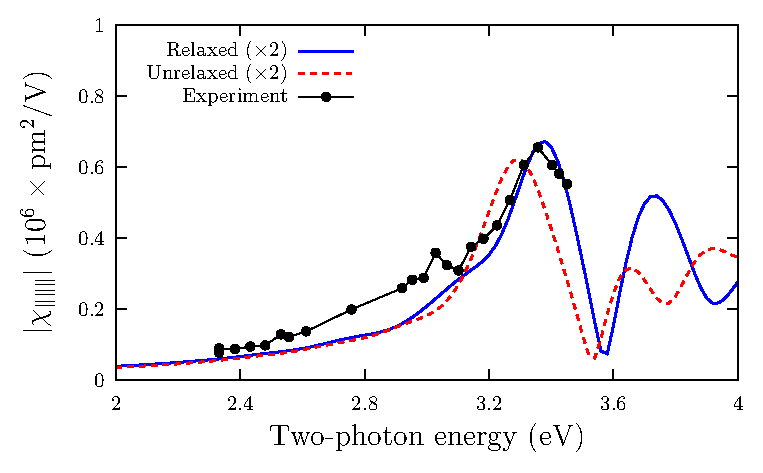
\includegraphics[width=0.48\textwidth]{plots/fig2}
\caption{(Color online) Comparison of
$\chi_{\parallel\parallel\parallel}(-2\omega;\omega,\omega)$ calculated using
relaxed and unrelaxed atomic positions, with the experimental data presented in
Ref. \onlinecite{hoferAPA96}. Theoretical curves are broadened with
$\sigma=0.075\,\text{eV}$. Experimental data was taken at 80 K.
\label{fig:Xxxx}}
\end{figure}

Therefore, the most accurate theoretical results are given by using relaxed
atomic positions for the calculation of
$\boldsymbol{\chi}(-2\omega;\omega,\omega)$. Although this process can be very
time consuming for large numbers of atoms, we consider it a crucial step. From a
numerical standpoint, this further demonstrates that SSHG is very sensitive to
the surface atomic positions. In particular, our results show that a correct
value of the Si-H bond length is not enough to obtain the most accurate SSHG
spectra, and that a full relaxation of the structure is required. Additionally,
the theory may coincide better with experiments that are conducted under very
low temperature conditions.


\subsection{Calculated \texorpdfstring{$\mathcal{R}_{pS}$}{RpS} compared to
experiment}\label{sec: RpS}

All calculations presented from this point on were done using the relaxed atomic
positions described in previous sections. We now move on to the theoretical SSHG
yield compared with experiment. We first compare the calculated
$\mathcal{R}_{pS}$ spectra with room temperature experimental data from Ref.
\onlinecite{mejiaPRB02}. We adhere to the experimental setup by taking an angle
of incidence $\theta=65^{\circ}$ and an azimuthal angle of $\phi=30^\circ$ with
respect to the $x$-axis. This azimuthal angle maximizes $r_{pS}$, as shown in
Eq. \eqref{eq:rpS}. In Fig. \ref{fig:RpS}, we see that all three models
reproduce the lineshape of the experimental spectrum which includes the peaks
corresponding to both the E$_{1}$ (3.4\,eV) and E$_{2}$ (4.3\,eV) critical
points of bulk silicon, and a smaller feature at around 3.8\,eV. The calculated
E$_{1}$ and E$_{2}$ peaks are redshifted by 0.1\,eV and 0.06\,eV, respectively,
compared with the experimental peaks.


\begin{figure}[b]
\centering
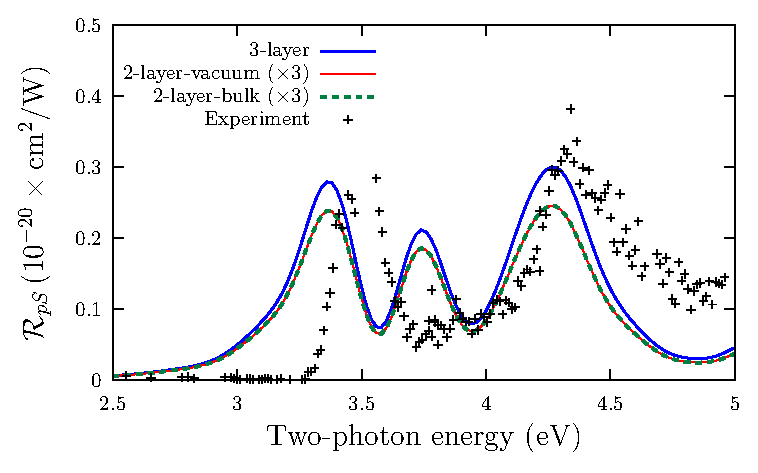
\includegraphics[width=0.48\textwidth]{plots/fig3}
\caption{(Color online) Comparison between theoretical models (see Table
\ref{tab:models}) and experiment for $\mathcal{R}_{pS}$, for
$\theta=65^{\circ}$. We use a scissors value of $\hbar\Delta = 0.7\,\text{eV}$.
All theoretical curves are broadened with $\sigma=0.075\,\text{eV}$.
Experimental data taken from Ref. \onlinecite{mejiaPRB02}, measured at room
temperature.
\label{fig:RpS}}
\end{figure}

The main issue to address here is the discrepancy between the intensity of the
E$_{1}$ peak. In the theoretical curves, the peaks differ only slightly in
overall intensity. Conversely, the experimental E$_{1}$ peak is significantly
smaller than the E$_{2}$ peak. This may be due to the effects of oxidation on
the surface. Ref. \onlinecite{bergfeldPRL04} features similar data to those of
Ref. \onlinecite{mejiaPRB02} but focuses on the effects of surface oxidation. We
can see that as time passes during the experiment, the surface becomes more
oxidized, and the E$_{1}$ peak diminishes substantially, as shown by the
experimental data taken 5 hours after initial H-termination. This may be enough
time to slightly reduce the E$_{1}$ peak intensity, as can be observed here.

In Fig. \ref{fig:mitchellRpS}, we compare the theoretical $\mathcal{R}_{pS}$
with experimental data from Ref. \onlinecite{mitchellSS01}; this data, however,
only encompasses the E$_{1}$ peaks, and was obtained at room temperature. We
consider an angle of incidence $\theta=45^\circ$ and an azimuthal angle
$\phi=30^\circ$ to match these experimental conditions. As in the previous
comparison, the E$_{1}$ peak is slightly redshifted compared to experiment. The
intensity of the theoretical yield is smaller than the experimental yield for
all three models. The measurements presented in Ref. \onlinecite{mitchellSS01}
were taken very shortly after the surface had been prepared, and the surface
itself was prepared with a high degree of quality and measured at room
temperature. Peak position compared to theory is slightly improved under these
conditions. As before, the 3-layer model is closer in intensity to
the experimental spectrum.

\begin{figure}[b]
\centering
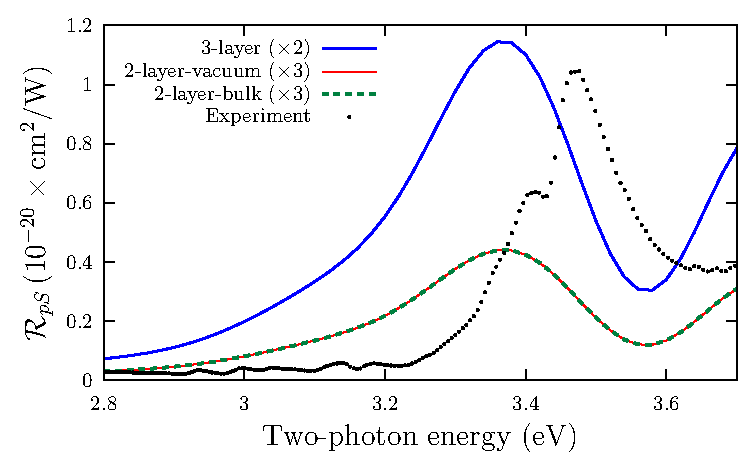
\includegraphics[width=0.48\textwidth]{plots/fig4}
\caption{(Color online) Comparison between theoretical models (see Table
\ref{tab:models}) and experiment for $\mathcal{R}_{pS}$, for $\theta=45^\circ$.
We use a scissors value of $\hbar\Delta = 0.7\,\text{eV}$. All theoretical
curves are broadened with $\sigma=0.075\,\text{eV}$. Experimental data taken
from Ref. \onlinecite{mitchellSS01}, measured at room temperature.
\label{fig:mitchellRpS}}
\end{figure}


We show in Fig.~\ref{fig:Xxxx} that our calculation for
$\chi_{\parallel\parallel\parallel}(-2\omega;\omega,\omega)$ coincides with the
measurement taken at a low temperature of 80 K. It is well known that
temperature causes shifting in the peak position of SSHG
spectra.\cite{dadapPRB97} As $\mathcal{R}_{pS}$ only depends on this component
(see Eq.~\eqref{eq:rpS}), the position of the theoretical peak should be correct
in Figs. \ref{fig:RpS} and \ref{fig:mitchellRpS}. We deduce that the difference
in peak position stems from the higher  temperature at which the experiments
were measured.


Both the 2-layer-vacuum and 2-layer-bulk models are identical and roughly 3
times smaller than the experiment. We can see from Eq. \eqref{eq:rpS} that
$\mathcal{R}_{pS}$ only has $1\omega$ terms ($\varepsilon_{\ell}(\omega)$ and
$k_{b}$). For both of these models, the fundamental fields are evaluated in the
bulk, which means that the only change to Eq. \eqref{eq:rpS} is that
$\varepsilon_{\ell}(\omega) \rightarrow \varepsilon_{b}(\omega)$. Additionally,
$\Gamma^{\ell}_{pS}$ also remains identical between the two models and has no
$2\omega$ terms in the denominator. Therefore, $r_{pS}$ is identical between
these two models. Ultimately, the intensity of the 3-layer model is the closest
to the experiment.

Per Eq. \eqref{eq:rpS}, the intensity of $\mathcal{R}_{pS}$ depends only on
$\chi_{\parallel\parallel\parallel}$, which is not affected by local field
effects.\cite{tancognedejean:tel-01235611} These effects are neglected in this
calculation, but $\mathcal{R}_{pS}$ maintains an accurate lineshape and provides
a good quantitative description of the experimental SSHG yield. We note that
both the calculated and experimental spectra show two-photon resonances at the
energies corresponding to the critical point transitions of bulk Si. We also see
that the SSHG yield drops rapidly to zero below E$_{1}$, which is consistent
with the absence of surface states due to the H saturation on the surface. This
observation holds true for all three polarization cases studied here.

Lastly, in Fig. \ref{fig:improvements} we provide an overview of the different
levels of approximation proposed in this article. All curves here were
calculated using the 3-layer model. The long dashed line depicts
the effect of excluding the contribution from the nonlocal part of the
pseduopotentials. This is consistent with the results reported in Ref.
\onlinecite{andersonPRB15}, where the exclusion of this term increases the
intensity of the components of $\boldsymbol{\chi}(-2\omega;\omega,\omega)$ by
approximately 15\% to 20\%. We also notice that the E$_{1}$ peak is larger than
the E$_{2}$ peak, contrasting with the experiment, where the E$_{1}$ peak is
smaller than E$_{2}$. Lastly, the thin solid line depicts the full calculation
with a scissors value of $\hbar\Delta = 0$. We notice that the spectrum is
almost rigidly redshifted as this H-saturated surface has no electronic surface
states.\cite{andersonPRB15} Thus, this demonstrates the importance of including
the scissors correction to accurately reproduce the experimental spectrum. In
summary, the inclusion of the contribution from the nonlocal part of the
pseudopotentials and the scissors operator on top of the 3-layer model produces
spectra with a lineshape and intensity that compare favorably with the
experimental data.

\begin{figure}[t]
\centering
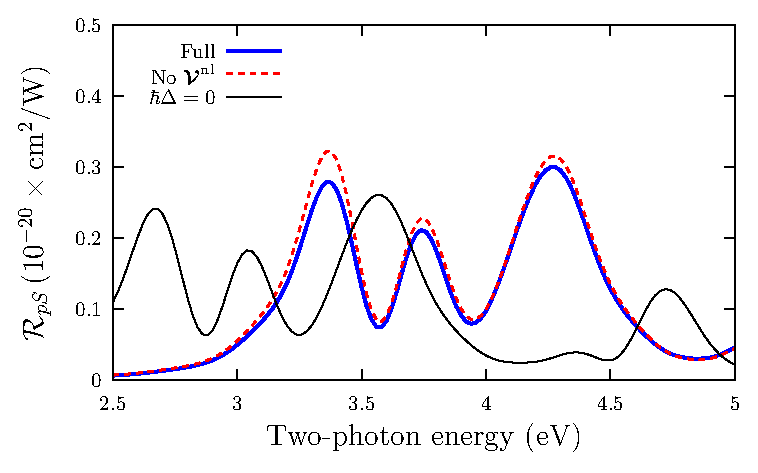
\includegraphics[width=0.48\textwidth]{plots/fig5}
\caption{(Color online) Calculated results for $\mathcal{R}_{pS}$ for the
different levels of approximation proposed in this article. All curves were
calculated using the 3-layer model. We take $\theta=65^{\circ}$ for this plot.
See text for full details. All curves are broadened with
$\sigma=0.075\,\text{eV}$.
\label{fig:improvements}}
\end{figure}


\subsection{Calculated \texorpdfstring{$\mathcal{R}_{sP}$}{RsP} compared to
experiment}\label{sec:RsP}

Next, we analyze and compare the calculated $\mathcal{R}_{sP}$ spectra with
experimental data from Ref. \onlinecite{mejiaPRB02}. We again adhere to the
experimental setup by taking an angle of incidence $\theta=65^{\circ}$ and an
azimuthal angle $\phi=30^\circ$. From Fig. \ref{fig:RsP}, we can immediately
appreciate that the overall intensity of $\mathcal{R}_{sP}$ is one order of
magnitude lower than $\mathcal{R}_{pS}$. The experimental data is far noisier
than in the other cases but we can still discern the E$_{1}$ and E$_{2}$ peaks.
As with our previous comparisons, the 3-layer model is the closest match in both
intensity and lineshape to the experimental spectrum. It produces a curve that
is very close to the experimental intensity with good proportional heights for
the calculated E$_{1}$ and E$_{2}$ peaks. In contrast, the 2-layer-vacuum model
is 100 times more intense than experiment and produces an enlarged E$_{2}$ peak.
The 2-layer-bulk model is ten times smaller with a very similar lineshape to the
3-layer model.

The differences between the 2-layer-vacuum and
2-layer-bulk models are not derived from Eq. \eqref{eq:rsP}, as the
$\varepsilon_{b}(2\omega)$ does not change and the second term vanishes for this
azimuthal angle of $\phi = 30$. However, $\Gamma^{\ell}_{sP}$ does cause a
significant change in the intensity as there is an $\varepsilon_{\ell}(2\omega)$
term in the denominator. This will become $\varepsilon_{v}(2\omega) = 1$ for the
2-layer-vacuum model, and $\varepsilon_{b}(2\omega)$ in the bulk
model. This accounts for the significant difference between the intensity of the
two models, while the lineshape remains mostly consistent.

At higher energies, the theoretical curve is blueshifted as compared to the
experiment. We consider that the likely explanation for this is the inclusion of
the scissor operator, which does not adequately correct the transitions
occurring at these higher energies. A full GW calculation would be well suited
for this task, but is beyond the scope of this paper.

\begin{figure}[t]
\centering
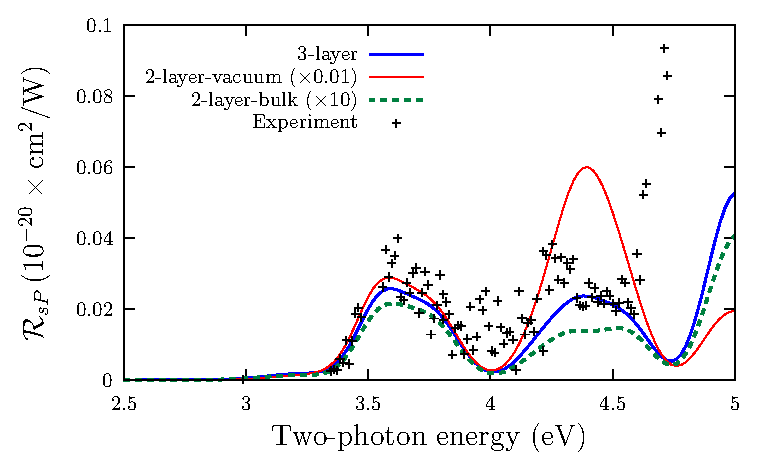
\includegraphics[width=0.48\textwidth]{plots/fig6}
\caption{(Color online) Comparison between theoretical models (see Table
\ref{tab:models}) and experiment for $\mathcal{R}_{sP}$, for
$\theta=65^{\circ}$. We use a scissors value of $\hbar\Delta = 0.7\,\text{eV}$.
All theoretical curves are broadened with $\sigma=0.075\,\text{eV}$.
Experimental data taken from Ref. \onlinecite{mejiaPRB02}, measured at room
temperature.
\label{fig:RsP}}
\end{figure}


\subsection{Calculated \texorpdfstring{$\mathcal{R}_{pP}$}{RpP} compared to
experiment}\label{sec:RpP}

We present $\mathcal{R}_{pP}$ compared to experimental data from Ref.
\onlinecite{mejiaPRB02} in Fig. \ref{fig:RpP}. We note that peak position for
the 3-layer model is similar to experiment with the overall intensity being only
two times larger. The E$_{2}$ peak is blueshifted by around 0.3\,eV, and the
yield does not go to zero after 4.75\,eV. The 2-layer-vacuum model produces a
spectrum with peak positions that are close to the experiment, but are 40 times
more intense. The calculated E$_{2}$ peak is similar, but the E$_{1}$ peak lacks
the sharpness present in the experiment. The 2-layer-bulk model is very close to
the lineshape of the 3-layer model, but with eight times less intensity. From
Eq. \eqref{eq:rpP}, we see that $\mathcal{R}_{pP}$ has several $2\omega$ terms
that will change between models; this will have a deep effect on the lineshape.
Additonally, $\Gamma^{\ell}_{pP}$ also has $\varepsilon_{\ell}(2\omega)$ in the
denominator, and so we have a significant difference in both lineshape and
intensity between the 2-layer-vacuum and the other two models. Again, as in the
previous sections for $\mathcal{R}_{pS}$ and $\mathcal{R}_{sP}$, the 3-layer
model is the closest in intensity to the experiment. Additionally, Ref.
\onlinecite{dadapPRB97} shows that low temperature measurements of
$\mathcal{R}_{pP}$ will blueshift the spectrum away from room temperature
measurements such as those shown in Figs. \ref{fig:RpP} and
\ref{fig:mitchellRpP}, and towards our theoretical results.

Reviewing Eq. \eqref{eq:rpP}, we see that $\mathcal{R}_{pP}$ is by far the most
involved calculation, since it includes all four nonzero components. In
particular, $\chi_{\perp\perp\perp}$ and $\chi_{\parallel\parallel\perp}$
include out-of-plane incoming fields. These are affected by local field
effects\cite{tancognedejean:tel-01235611} that reveal the inhomogeneities in the
material, which are by far more prevalent perpendicular to the surface than in
the surface plane. This can be evidenced for Si, as Reflectance Anisotropy
Spectroscopy (RAS) measurements are well described by \emph{ab initio}
calculations neglecting local field effects.\cite{palummoPRB99, gaalPRB09} It is
therefore expected that the out-of-plane components will be more sensitive to
the inclusion of local fields. These will not change the transition energies,
only their relative weights of the resonant
peaks,\cite{tancognedejean:tel-01235611} but including these effects is
challenging to compute,\cite{nicolasPRB15} and beyond the scope of this paper.

We speculate that $\mathcal{R}_{pP}$ requires the
proper inclusion of these effects in order to accurately describe the
experimental peaks.

\begin{figure}[b]
\centering 
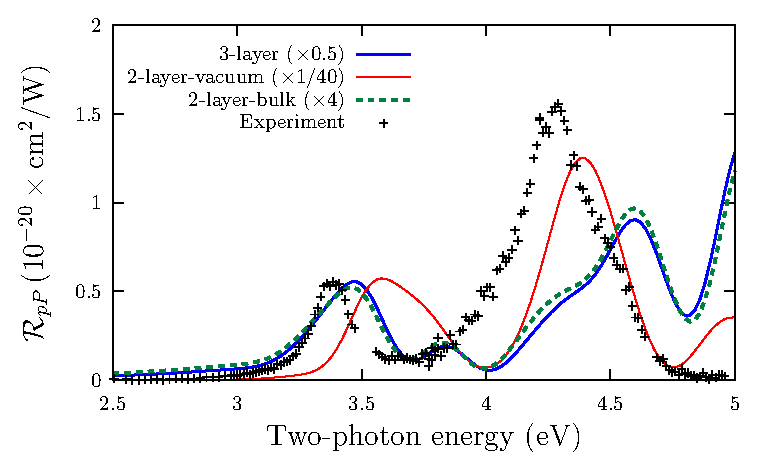
\includegraphics[width=0.48\textwidth]{plots/fig7}
\caption{(Color online) Comparison between theoretical models (see Table
\ref{tab:models}) and experiment for $\mathcal{R}_{pP}$, for
$\theta=65^{\circ}$. We use a scissors value of $\hbar\Delta = 0.7\,\text{eV}$.
All theoretical curves are broadened with $\sigma=0.075\,\text{eV}$.
Experimental data taken from Ref. \onlinecite{mejiaPRB02}, measured at room
temperature.
\label{fig:RpP}}
\end{figure}

In Fig. \ref{fig:mitchellRpP} we compare to Ref. \onlinecite{mitchellSS01}. The
3-layer model is, as before, close to the experiment in both peak position and
intensity. Intensity is almost the same the experimental value. This provides a
more compelling argument against the 2-layer-vacuum model than Fig.
\ref{fig:RpP}. The 2-layer-vacuum model is 20 times more intense and blueshifted
by around 0.1\,eV. As mentioned before, this surface is of very high quality
with measurements taken shortly after surface preparation. As before, the
2-layer-bulk model is intermediate between the other two models in both
intensity and lineshape. Under these conditions, the 3-layer model very
accurately reproduces the E$_{1}$ peak over the 2-layer-vacuum and 2-layer-bulk
models.

\begin{figure}[t]
\centering
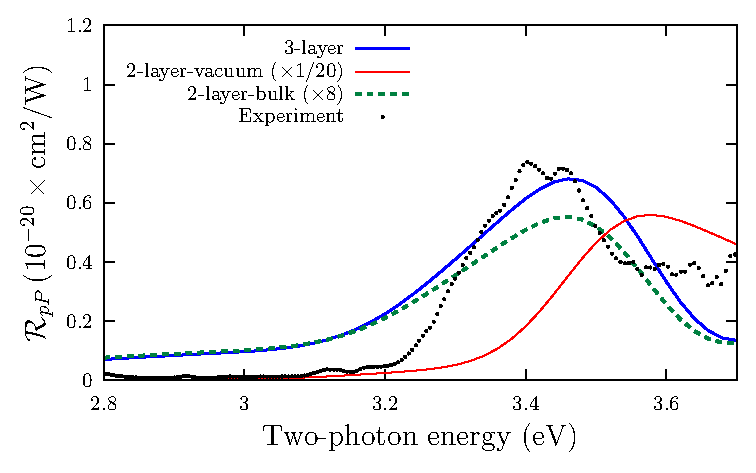
\includegraphics[width=0.48\textwidth]{plots/fig8}
\caption{(Color online) Comparison between theoretical models (see Table
\ref{tab:models}) and experiment for $\mathcal{R}_{pP}$, for
$\theta=45^{\circ}$. We use a scissors value of $\hbar\Delta = 0.7\,\text{eV}$.
All theoretical curves are broadened with $\sigma=0.075\,\text{eV}$.
Experimental data taken from Ref. \onlinecite{mitchellSS01}, measured at room
temperature.
\label{fig:mitchellRpP}}
\end{figure}

Lastly, for linear optics and SHG, $GW$ transition energies are needed. Doing a
Bethe-Salpeter calculation for SSHG will improve the position and the amplitude
of the peaks, but is far beyond current capabilities.\cite{puff} We did not
adjust the value of the scissors shift, as we want to keep our calculation at
the {\em ab initio} level. We remark again that the choice of $\hbar\Delta=0.7$
eV for the scissors shift comes from a $GW$ calculation.\cite{liPRB10} As
explained in Fig. \ref{fig:improvements}, the lack of surface states causes an
almost rigid shift of the spectra by applying the scissors correction. We have
checked that it is not possible to have a single scissors value that can
reproduce the energy positions of both the E$_{1}$ and the E$_{2}$ peaks. Of
course, the experimental temperature at which the spectra is measured should be
taken into account in a more complete formulation. However, we have restricted
our calculation to $T=0$ K.


\section{Conclusions}\label{sec:conclusions}

We have presented new \emph{ab initio} LDA calculations for SSHG that are in
good quantitative agreement with experimental SSHG spectra for the
Si(111)(1$\times$1):H surface. These calculations include contributions not
previously considered in a single formulation, to wit, (i) the scissors
correction, (ii) the contribution of the nonlocal part of the pseudopotentials,
and (iii) the cut function used to extract the surface response, all within the
independent particle approximation. We also revised the 3-layer model for the
SSHG yield where the nonlinear polarization,
$\boldsymbol{\mathcal{P}}(2\omega)$, and the fundamental fields are taken within
a small layer $\ell$ below the surface of the material. This model reproduces
key spectral features and yields an intensity closer to the experiment for all
cases of $\mathcal{R}_{\mathrm{iF}}$. We consider it an upgrade over the much
reviewed 2-layer model\cite{mizrahiJOSA88}, and it comes with very little added
computational expense. Additionally, we have compared these two models with
another definition of the 2-layer model, where both
$\boldsymbol{\mathcal{P}}(2\omega)$ and the fundamental fields are considered
inside the bulk of the material. We found that this model yields an intensity
lower than the 3-layer model, but far closer than the 2-layer-vacuum model.
Lineshape is very similar between the 3-layer and 2-layer-bulk models.
Therefore, we consider that the 3-layer model offers the closest comparison to
experiment, while the 2-layer-bulk model offers a reasonable compromise between
the 3-layer and 2-layer-vacuum models.

This study affords us an interesting view of both the theoretical and
experimental aspects of SSHG studies. On the theoretical side, we have shown the
importance of using relaxed atomic positions to more accurately calculate the
nonlinear susceptibility tensor. The intensity of these spectra is greatly
improved when compared to previous works.\cite{mejiaPRB02} We also postulate
that the lack of local field effects in the theory is a serious shortcoming, but
in this case, it only affects two of the
$\boldsymbol{\chi}(-2\omega;\omega,\omega)$ components.

Concerning the experiments, we show that surface preparation and quality are
important for better results. The approach for calculating the SSHG yield
presented here finds closer agreement with surfaces that are freshly prepared
with little or no oxidation, and with measurements taken at low temperatures.

Overall, this newly implemented framework for calculating
$\boldsymbol{\chi}(-2\omega;\omega,\omega)$ and $\mathcal{R}$ focused on the
well-known Si(111)(1$\times$1):H surface provides a compelling benchmark for
SSHG studies. We are confident that this work can be applied directly to many
other surfaces of interest.


\section{Acknowledgements}\label{sec:acknowledgements}

B.S.M. acknowledges the Laboratoire des Solides Irradi\'es (Ecole Polytechnique,
Palaiseau, France) for the support and hospitality during a sabbatical year.
B.S.M. acknowledges partial support from CONACYT-M\'exico Grant 153930. S.M.A.
gratefully acknowledges full support from CONACYT-M\'exico scholarship 349278.


\bibliography{ref}

\end{document}
